\documentclass[enabledeprecatedfontcommands,fontsize=12pt,paper=a4,twoside]{scrartcl}


\newcommand{\grad}{\ensuremath{^{\circ}} }
\renewcommand{\strut}{\vrule width 0pt height5mm depth2mm}

\usepackage{longtable}
\usepackage[utf8]{inputenc}
\usepackage[T1]{fontenc}
\usepackage[final]{pdfpages}
% obere Seitenränder gestalten können
\usepackage{fancyhdr}
\usepackage{moreverb}
% Graphiken als jpg, png etc. einbinden können
\usepackage{graphicx}
\usepackage[normalem]{ulem}
\useunder{\uline}{\ul}{}
\usepackage{stmaryrd}
% Floats Objekte mit [H] festsetzen
\usepackage{float}
% setzt URL's schön mit \url{http://bla.laber.com/~mypage}
\usepackage{url}
% Externe PDF's einbinden können
\usepackage{pdflscape}
% Verweise innerhalb des Dokuments schick mit " ... auf Seite ... "
% automatisch versehen. Dazu \vref{labelname} benutzen
\usepackage[ngerman]{varioref}
\usepackage[ngerman]{babel}
\usepackage{ngerman}
% Bibliographie
\usepackage{bibgerm}
% Tabellen
\usepackage{tabularx}
\usepackage{supertabular}
\usepackage[colorlinks=true, pdfstartview=FitV, linkcolor=blue,
            citecolor=blue, urlcolor=blue, hyperfigures=true,
            pdftex=true]{hyperref}
\usepackage{bookmark}
\usepackage{rotating}
\usepackage{float}

\hyphenation{Arbeits-paket}

% Damit Latex nicht zu lange Zeilen produziert:
\sloppy
%Uneinheitlicher unterer Seitenrand:
%\raggedbottom

% Kein Erstzeileneinzug beim Absatzanfang
% Sieht aber nur gut aus, wenn man zwischen Absätzen viel Platz einbaut
\setlength{\parindent}{0ex}

% Abstand zwischen zwei Absätzen
\setlength{\parskip}{1ex}

% Seitenränder für Korrekturen verändern
\addtolength{\evensidemargin}{-1cm}
\addtolength{\oddsidemargin}{1cm}

\bibliographystyle{gerapali}

% Lustige Header auf den Seiten
  \pagestyle{fancy}
  \setlength{\headheight}{70.55003pt}
  \fancyhead{}
  \fancyhead[LO,RE]{Software--Projekt 2\\ WiSe 2019/2020
  \\Architekturbeschreibung}
  \fancyhead[LE,RO]{Seite \thepage\\\slshape \leftmark\\\slshape \rightmark}

%Unicode Minuszeichen deklarieren, um es nicht überall austauschen zu müssen
\DeclareUnicodeCharacter{2212}{-}

%
% Und jetzt geht das Dokument los....
%

\begin{document}

% Lustige Header nur auf dieser Seite
  \thispagestyle{fancy}
  \fancyhead[LO,RE]{ }
  \fancyhead[LE,RO]{Universität Bremen\\FB 3 -- Informatik\\
  Prof. Dr. Rainer Koschke \\TutorIn: Marcel Steinbeck}
  \fancyfoot[C]{}

% Start Titelseite
  \vspace{3cm}

  \begin{minipage}[H]{\textwidth}
  \begin{center}
  \bf
  \Large
  Software--Projekt 2 WiSe 2019/2020\\
  \smallskip
  \small
  VAK 03-BA-901.02\\
  \vspace{3cm}
  \end{center}
  \end{minipage}
  \begin{minipage}[H]{\textwidth}
  \begin{center}
  \vspace{1cm}
  \bf
  \Large Architekturbeschreibung\\ Data Colorado\\
  \vfill
  \end{center}
  \centering
  
\includegraphics[width=0.4\textwidth]{UML/Logo.png}\\
  \end{minipage}
  \vfill
  \begin{minipage}[H]{\textwidth}
  \begin{center}
  \sf
  \begin{tabular}{lr}
  Liam Hurwitz & hurwitz@tzi.de \\
  Kevin Santiago Rodriguez Rey & kev\textunderscore rey@tzi.de \\
  Fabian Kehlenbeck & fkehlenb@tzi.de \\
  Aaron Rudkowski & rudkowsk@tzi.de \\
  Samuel Nejati Masouleh & samnej@tzi.de \\
  Leonard Haddad & s\textunderscore xsipo6@tzi.de \\  
\end{tabular}
  \\ ~
  \vspace{2cm}
  \\
  \it Abgabe: 08.03.2020 --- Version 1.0\\ ~
  \end{center}
  \end{minipage}

% Ende Titelseite

% Start Leerseite

\newpage

  \thispagestyle{fancy}
  \fancyhead{}
  \fancyhead[LO,RE]{Software--Projekt \\  2019/2020
  \\Benutzerhandbuch}
  \fancyhead[LE,RO]{Seite \thepage\\\slshape \leftmark\\~}
  \fancyfoot{}
  \renewcommand{\headrulewidth}{0.4pt}
  \tableofcontents

\newpage

  \fancyhead[LE,RO]{Seite \thepage\\\slshape \leftmark\\\slshape \rightmark}


%%%%%%%%%%%%%%%%%%%%%%%%%%%%%%%%%%%%%%%%%%%%%%%%%%%%%%%%%%%%%%%%%%%%%%%%


\section*{Version und Änderungsgeschichte}

{\em Die aktuelle Versionsnummer des Dokumentes sollte eindeutig und gut zu
identifizieren sein, hier und optimalerweise auf dem Titelblatt.}

\begin{tabular}{ccl}
Version & Datum & Änderungen \\
\hline
%0.1 & TT.MM.JJJJ & Dokumentvorlage als initiale Fassung kopiert \\
0.1 & 03.03.2020 & Erste Schritte \\
0.2 & 03.03.2020 & Administrator \\
\end{tabular}


%%%%%%%%%%%%%%%%%%%%%%%%%%%%%%%%%%%%%%%%%%%%%%%%%%%%%%%%%%%%%%%%%%%%%%%%

\newpage
\section{Einführung}
\subsection{Haftungsbeschränkung}
\subsection{Addressierte Leser}
\subsection{Zweck}
\subsection{Verwandte Dokumente}
\subsection{Information über die Verwendung des Dokuments}
\subsection{Instruktionen für Problemberichte}

%%%%%%%%%%%%%%%%%%%%%%%%%%%%%%%%%%%%%%%%%%%%%%%%%%%%%%%%%%%%%%%%%%%%%%%%

\newpage
\section{Übersicht}

%%%%%%%%%%%%%%%%%%%%%%%%%%%%%%%%%%%%%%%%%%%%%%%%%%%%%%%%%%%%%%%%%%%%%%%%

\newpage
\section{Erste Schritte für Anwender}
\subsection{Anmeldung}
\subsection{Abmeldung}
\subsection{Sprachauswahl}
\subsection{Navigationsleiste}

%%%%%%%%%%%%%%%%%%%%%%%%%%%%%%%%%%%%%%%%%%%%%%%%%%%%%%%%%%%%%%%%%%%%%%%%

\newpage
\section{Farbige Zustände für Administratoren}
\subsection{Installation der Applikation}
\subsection{Benutzer}
Die Aktionen bezüglich der Benutzer des Systems können Sie unter dem Unterpunkt Nutzer Verwalten aufrufen. 
Hier haben Sie eine Tabelle, die alle Benutzer anzeigt, die aktuell im System vorhanden sind. Die Benutzer werden für bessere Übersicht seitenweise angezeigt, mit den Knöpfen oberhalb und unterhalb der Tabelle können Sie durch diese Seiten navigieren.\\
 In dieser Tabelle können Sie durch drücken auf den Knopf Löschen einen User aus dem System entfernen.  
\begin{figure}[h!]
\begin{center}
 
\includegraphics[width=\textwidth]{screenshots/admin/nutzerloeschen.png}
  \caption{Nutzer erfolgreich gelöscht}
  \label{fig:boat2}
\end{center}
\end{figure}
Durch drücken auf den Knopf Bearbeiten werden die Daten des Users in das Formular oberhalb der Tabelle geschrieben, wo Sie Änderungen vornehmen können. 
Bitte beachten Sie, in dem Feld Email nur Eingaben in der Form []@[].[] einzugeben, wobei die Endung länger als zwei Zeichen sein muss. Des weiteren dürfen für die Telefonnummer nur Zahlen eingegeben werden. Sollten Sie Fehler in den Eingaben machen, werden Ihnen die fehlerhaften Felder rot unterlegt. Die ID eines Benutzers können Sie nicht bearbeiten, da diese vom System verwaltet werden. \\
Mit Drücken auf Reset werden die bisher gespeicherten Daten wieder hergestellt. Mit Drücken auf Speichern können Sie Ihre Änderungen speichern. \\
//TODO Bild

Über der Tabelle befindet sich ein Formular, in dem Sie die Daten für einen neuen Benutzer eingeben können. Wenn sie alle Daten eingegeben haben, klicken Sie auf Speichern, um den Benutzer zu speichern. Die ID müssen Sie nicht selber eingeben, da sie vom System generiert wird. 
Hier gelten die gleichen Beschränkungen wie oben für die Bearbeitung von Benutzern genannt. 
\begin{figure}[h!]
\begin{center}
 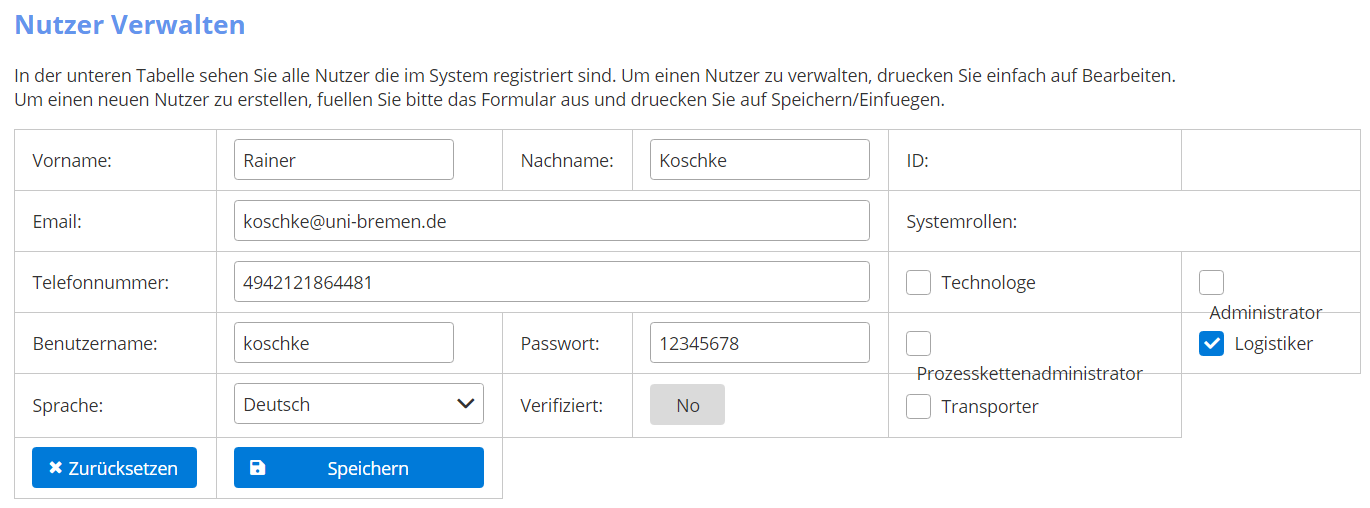
\includegraphics[width=\textwidth]{screenshots/admin/nutzerformularausgefuellt.png}
  \caption{Nutzerformular ausgefüllt}
  \label{fig:boat3}
\end{center}
\end{figure}
Bei erfolgreicher Erstellung eines Benutzer werden Sie eine Nachricht am rechten Rand des Fensters sehen, der neue Benutzer wird in der Tabelle erscheinen und eine Email bekommen. 
\begin{figure}[h!]
\begin{center}
 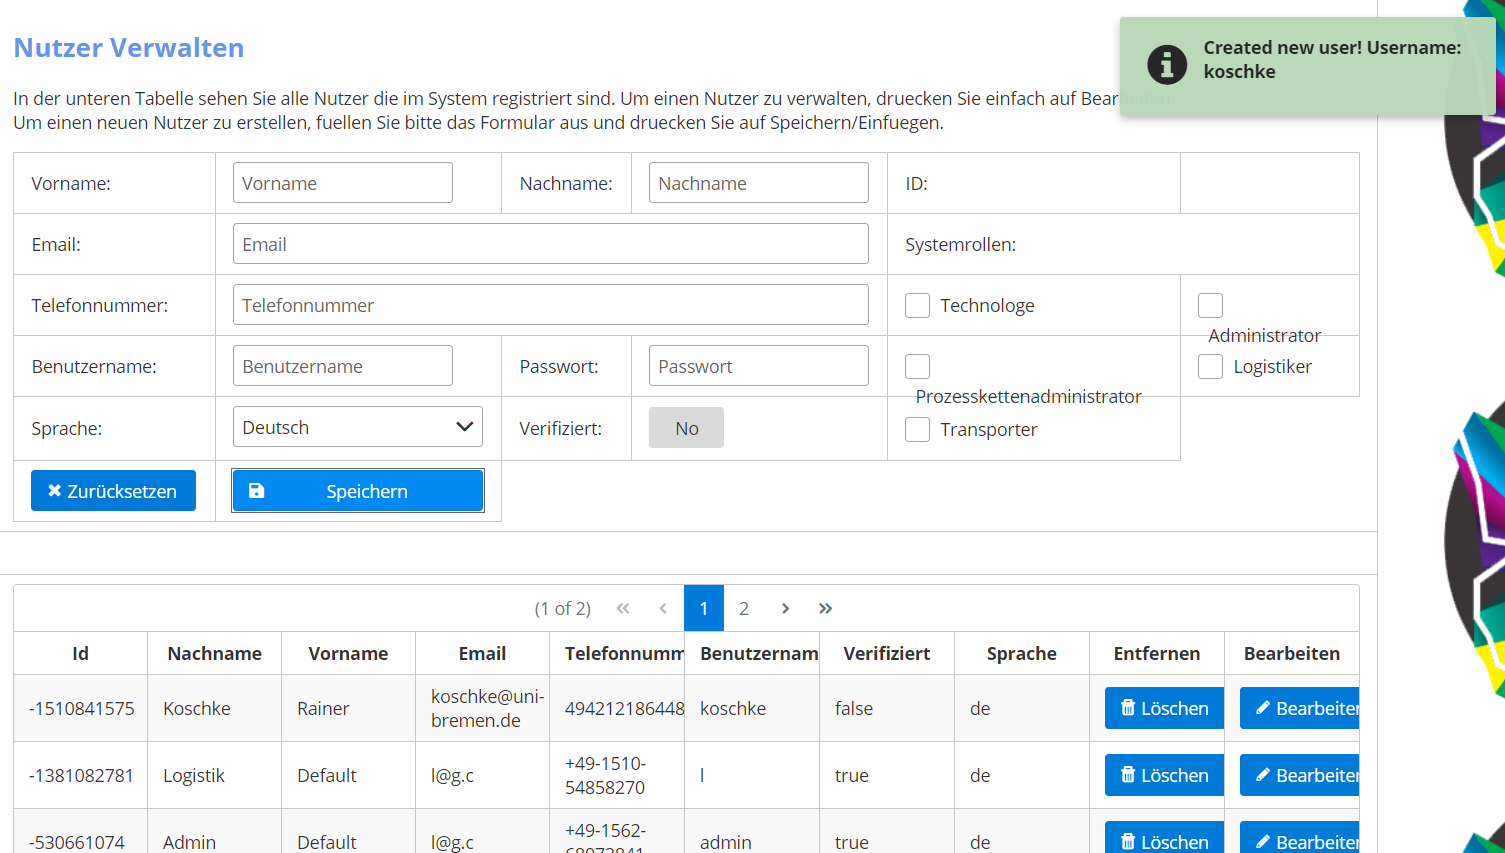
\includegraphics[width=\textwidth]{screenshots/admin/nutzererfolgreich.png}
  \caption{Nutzer erfolgreich gespeichert}
  \label{fig:boat1}
\end{center}
\end{figure}
Wenn sie das Formular zurücksetzen wollen, drücken Sie auf Reset. 
\subsection{Experimentierstationen}
\subsection{Globale Einstellungen}
\subsection{Backup der Systemdaten}

%%%%%%%%%%%%%%%%%%%%%%%%%%%%%%%%%%%%%%%%%%%%%%%%%%%%%%%%%%%%%%%%%%%%%%%%

\newpage
\section{Farbige Zustände für andere Mitarbeiter}
\subsection{Prozesskettenadministrator}
\subsubsection{Übersicht über Prozessschritte}
\subsubsection{Übersicht über dynamische Abläufe}
\subsubsection{Übersicht über Prozessketten}
\subsubsection{Übersicht über Aufträge}
\subsection{Logistiker}
\subsubsection{Übersicht über Träger}
\subsubsection{Übersicht über freigegeben Aufträge}
\subsubsection{Übersicht über Probenmengen}
\subsubsection{Übersicht über archivierte Proben}
\subsubsection{Übersicht über Probenstandorte}
\subsection{Technologe}
\subsubsection{Übersicht über Experimentierstationen}
\subsubsection{Übersicht über aktuelle Arbeitsarufträge}
\subsubsection{Übersicht über angekündigte Abeitsaufträge}
\subsubsection{Aktualisieren des Zustands eines Arbeitrauftrags}
\subsubsection{Probenupload}
\subsubsection{Proben melden}
\subsubsection{Experimentierstation melden}
\subsubsection{Kommentare}
\subsection{Transporter}
\subsubsection{Übersicht über anstehende Transportaufträge}
\subsubsection{Probenverlust melden}

%%%%%%%%%%%%%%%%%%%%%%%%%%%%%%%%%%%%%%%%%%%%%%%%%%%%%%%%%%%%%%%%%%%%%%%%

\newpage
\section{Probleme und Ursachen}

%%%%%%%%%%%%%%%%%%%%%%%%%%%%%%%%%%%%%%%%%%%%%%%%%%%%%%%%%%%%%%%%%%%%%%%%

\end{document}